\documentclass[conference]{IEEEtran}

\usepackage[utf8]{inputenc}
\usepackage[T1]{fontenc}
\usepackage{mathptmx}
\usepackage[spanish,es-tabla,es-noshorthands,es-nolayout]{babel}
\addto\captionsspanish{\renewcommand{\figurename}{Fig.}\renewcommand{\refname}{Referencias}}
\usepackage{amsmath}
\usepackage{graphicx}
\usepackage{booktabs}
\usepackage{array}
\usepackage{textcomp}
\usepackage{cite}
\usepackage{url}
\usepackage{microtype}

\graphicspath{{figs/}}
\hyphenation{Cher-nobyl Lagu-na}

\begin{document}
\renewcommand{\IEEEkeywordsname}{Palabras clave}

\title{Reconstrucci\'on geoespacial de la deposici\'on de $^{137}$Cs tras Chernobyl en Europa Central: distancia, relieve y decaimiento, con una extensi\'on a Laguna Verde}

\author{\IEEEauthorblockN{Ian A. Sandoval-Valderr\'abano}
\IEEEauthorblockA{\textit{Facultad de Ingenier\'ia}\\
\textit{Benem\'erita Universidad Aut\'onoma de Puebla}\\
Puebla, M\'exico}}

\maketitle
\begin{abstract}
La deposici\'on de cesio-137 ($^{137}$Cs) tras el accidente de Chernobyl (1986) en Europa no sigui\'o un patr\'on de atenuaci\'on con la distancia. Este trabajo describe un flujo de an\'alisis geoespacial para contrastar la intensidad de la deposici\'on con la distancia a la fuente y con el relieve, y lo aplica a Europa Central. La deposici\'on de mayo de 1986, tomada del atlas europeo de De Cort et al., se proyecta a un sistema acimutal equivalente de Lambert y se resume por pa\'is mediante estad\'istica zonal en tres clases (menos de 6,000; de 6,000 a 28,000; y de 28,000 a 120,000~Bq/m$^2$). Se calcula la distancia geod\'esica (WGS84) de cada centroide a la central. La Rep\'ublica Checa, Austria y Eslovenia, a 1,061--1,265~km, quedan en la clase m\'as alta, mientras que Italia y Suiza, a distancias casi iguales (1,660 y 1,671~km), quedan en clases distintas; esto es coherente con un efecto de barrera de los Alpes, que aqu\'i se eval\'ua solo de forma visual. El decaimiento radiactivo deja el 45.6~\% del inventario en 2020 y alrededor del 40~\% en 2026, y los picos de 120,000~Bq/m$^2$ bajar\'ian de 37,000~Bq/m$^2$ hacia 2037. Se se\~nala un posible sesgo al alza en los promedios nacionales. El mismo enfoque se traslada a la Central Nucleoel\'ectrica de Laguna Verde (Veracruz): dentro de la zona de ingesti\'on de 80~km el terreno asciende unos 2,200~m, con una pendiente media de unos 27~m/km, casi el doble de la de la vertiente norte alpina en la misma malla.
\end{abstract}

\begin{IEEEkeywords}
Cesio-137, Chernobyl, deposici\'on h\'umeda, forzamiento orogr\'afico, sistemas de informaci\'on geogr\'afica, decaimiento radiactivo, Laguna Verde.
\end{IEEEkeywords}

\section{Introducci\'on}
El 26 de abril de 1986 el accidente de la unidad 4 de la central de Chernobyl liber\'o a la atm\'osfera grandes cantidades de radionucleidos. Las estimaciones recientes sit\'uan la emisi\'on de $^{137}$Cs en $85\pm26$~PBq, con una liberaci\'on de unos diez d\'ias y un segundo m\'aximo entre el 2 y el 5 de mayo~\cite{oecd2002}. Por su vida media de 30.05 a\~nos~\cite{pearce2008}, el $^{137}$Cs es el principal indicador de la contaminaci\'on residual: m\'as de 200,000~km$^2$ de Europa superaron el umbral de 37~kBq/m$^2$ que define las zonas contaminadas~\cite{iaea2006}.

La deposici\'on no disminuy\'o de forma regular con la distancia. Aunque m\'as del 70~\% del \'area contaminada se concentra en Bielorrusia, Rusia y Ucrania~\cite{iaea2006}, pa\'ises lejanos como Austria recibieron una fracci\'on apreciable del total~\cite{izrael1996}. La causa principal fue la lluvia durante el paso de la nube, porque las part\'iculas finas viajaron lejos y se depositaron sobre todo con la precipitaci\'on~\cite{oecd2002}. En ese proceso el relieve puede ser importante, ya que las monta\~nas fuerzan el ascenso del aire h\'umedo e intensifican la lluvia en las vertientes de barlovento~\cite{garcia2003}.

El objetivo es contrastar, con un flujo de trabajo sencillo y repetible, la intensidad de la deposici\'on de $^{137}$Cs con la distancia a la fuente y con el relieve en Europa Central, y trasladar la idea al entorno de la Central Nucleoel\'ectrica de Laguna Verde (Veracruz). El trabajo aporta:
\begin{itemize}
\item la intensidad media de $^{137}$Cs por pa\'is, comparada con la distancia geod\'esica a la central;
\item una lectura cartogr\'afica del posible efecto de barrera de los Alpes;
\item la evoluci\'on del inventario en 2020 y 2026 por decaimiento f\'isico;
\item una revisi\'on de los resultados con valores publicados;
\item un an\'alisis morfoestructural preliminar del entorno de Laguna Verde.
\end{itemize}

\section{Marco te\'orico}
\subsection{El $^{137}$Cs como trazador}
El $^{137}$Cs es un producto de fisi\'on que decae por emisi\'on beta con una vida media recomendada de $10\,976\pm30$~d\'ias, es decir, 30.05~a\~nos~\cite{pearce2008}. Su permanencia en el suelo durante d\'ecadas lo hace la referencia para cartografiar la contaminaci\'on de Chernobyl. Los atlas europeos expresan la deposici\'on en Bq/m$^2$ y consideran contaminadas las zonas con m\'as de 37~kBq/m$^2$~\cite{iaea2006}. Seg\'un Izrael et al.~\cite{izrael1996}, cerca del 6~\% del territorio europeo recibi\'o m\'as de 20~kBq/m$^2$ y alrededor del 2~\% m\'as de 40~kBq/m$^2$.

\subsection{Deposici\'on seca y h\'umeda}
La deposici\'on seca depende del contacto directo entre la nube y la superficie; la h\'umeda ocurre cuando la precipitaci\'on arrastra las part\'iculas al suelo. En Chernobyl, que lloviera o no durante el paso de la nube explica buena parte de la variabilidad espacial~\cite{oecd2002}. En Voivodina (Serbia), por ejemplo, la mejor correlaci\'on entre precipitaci\'on y $^{137}$Cs en el suelo se obtuvo para los periodos lluviosos de mayo de 1986~\cite{kalkan2021}.

\subsection{Forzamiento orogr\'afico}
Una masa de aire h\'umedo que encuentra una cordillera asciende, se enfr\'ia adiab\'aticamente y descarga su humedad en la vertiente de barlovento; en la opuesta se forma una sombra pluviom\'etrica~\cite{garcia2003}. Si el aire transporta part\'iculas radiactivas, el mismo mecanismo puede concentrar la deposici\'on h\'umeda en las laderas expuestas y reducirla a sotavento.

\subsection{Contexto meteorol\'ogico de 1986}
Al principio el viento llev\'o la nube hacia el noroeste, con deposici\'on en Escandinavia, los Pa\'ises Bajos, B\'elgica y Gran Breta\~na. Despu\'es la pluma gir\'o hacia el sur y alcanz\'o Europa Central, el norte del Mediterr\'aneo y los Balcanes~\cite{oecd2002}. La nube lleg\'o a Austria unas 80~horas despu\'es del accidente. El 29 de abril se registraron hasta 20~mm de lluvia en Pongau y Lungau, y el 30 de abril hasta 25~mm en Hausruck y Traunviertel, mientras que en el este de Austria llovi\'o muy poco~\cite{geosphere2026}.

\section{Datos y metodolog\'ia}
\subsection{Datos}
Se emplearon cinco conjuntos de datos:
\begin{itemize}
\item la matriz de deposici\'on de $^{137}$Cs de 1986, basada en el atlas de De Cort et al.~\cite{decort1998};
\item el modelo digital de elevaci\'on (DEM) SRTM GL3, de 3~segundos de arco (unos 90~m), obtenido en OpenTopography~\cite{srtm2013};
\item los l\'imites pol\'iticos y la l\'inea de costa de Natural Earth, escala 1:10\,m~\cite{ne10};
\item la topograf\'ia global ETOPO1~\cite{etopo1}, remuestreada a 10~minutos de arco~\cite{fatiando}, para los perfiles comparativos;
\item las zonas del Plan de Emergencia Radiol\'ogica Externo (PERE) de Laguna Verde~\cite{pere2011}.
\end{itemize}

\subsection{Proyecci\'on y representaci\'on}
Los conjuntos se proyectaron al sistema m\'etrico acimutal equivalente de Lambert (GRS80, EPSG:3035). Al conservar las \'areas, esta proyecci\'on permite la estad\'istica zonal sin distorsionar las superficies. La deposici\'on se clasific\'o entre 0 y 120,000~Bq/m$^2$ y se superpuso, con 40~\% de transparencia, sobre el relieve sombreado del DEM, para comparar visualmente la distribuci\'on del is\'otopo con la forma del terreno.

\subsection{Estad\'istica zonal}
La matriz de deposici\'on se cruz\'o con los l\'imites pol\'iticos para obtener la intensidad media de $^{137}$Cs en cada pa\'is. Las medias se agruparon en tres clases: menos de 6,000; de 6,000 a 28,000; y de 28,000 a 120,000~Bq/m$^2$.

\subsection{Distancia geod\'esica a la fuente}
Para cada pa\'is se calcul\'o el centroide de su pol\'igono en la proyecci\'on equivalente; para Francia se us\'o solo el territorio metropolitano. Luego se obtuvo la distancia geod\'esica sobre el elipsoide WGS84 entre la central de Chernobyl ($51.389^\circ$\,N, $30.100^\circ$\,E) y cada centroide. El mismo c\'alculo se aplic\'o a ciudades representativas.

\subsection{Evoluci\'on temporal}
El inventario remanente se estim\'o con la ley de decaimiento
\begin{equation}
A(t)=A_0\,2^{-t/T_{1/2}},
\label{eq:decay}
\end{equation}
donde $A_0$ es la actividad depositada en mayo de 1986, $t$ el tiempo transcurrido en a\~nos y $T_{1/2}=30.05$~a\~nos~\cite{pearce2008}. Solo se considera el decaimiento f\'isico; no se incluyen la migraci\'on vertical en el suelo, la erosi\'on ni la absorci\'on por la vegetaci\'on.

\subsection{An\'alisis morfoestructural de Laguna Verde}
Sobre la topograf\'ia ETOPO1 a $10'$ se trazaron las zonas del PERE como c\'irculos geod\'esicos centrados en la central ($19.7206^\circ$\,N, $96.4064^\circ$\,O): la Zona V\'ia Pluma (ZVP) de 16~km y la Zona V\'ia Ingesti\'on (ZVI) de 80~km~\cite{pere2011}. Se extrajeron dos perfiles, muestreados cada 2~km con interpolaci\'on bilineal: uno norte--sur a lo largo de $12^\circ$\,E, entre $49^\circ$\,N y $45.3^\circ$\,N, que cruza los Alpes orientales, y otro desde la central hacia el Cofre de Perote, con acimut de $252^\circ$. Ambos salen de la misma malla y son comparables entre s\'i, aunque la resoluci\'on de $10'$ suaviza las cumbres.

\section{Resultados}
\subsection{Distribuci\'on de la deposici\'on}
La Fig.~\ref{fig:dep} muestra la deposici\'on inicial en Europa Central. La mayor concentraci\'on est\'a en el sur de Baviera y en el piedemonte septentrional de los Alpes, con valores de hasta 120,000~Bq/m$^2$, adem\'as de n\'ucleos aislados en el resto del \'area. El patr\'on coincide con lo reportado por la Oficina Federal de Protecci\'on Radiol\'ogica de Alemania (BfS): al sur del Danubio y en el Bosque B\'avaro se midieron hasta 100,000~Bq/m$^2$ o m\'as, mientras que en la llanura del norte de Alemania la deposici\'on rara vez super\'o los 4,000~Bq/m$^2$~\cite{bfs2026}.

\begin{figure*}[t]
\centering
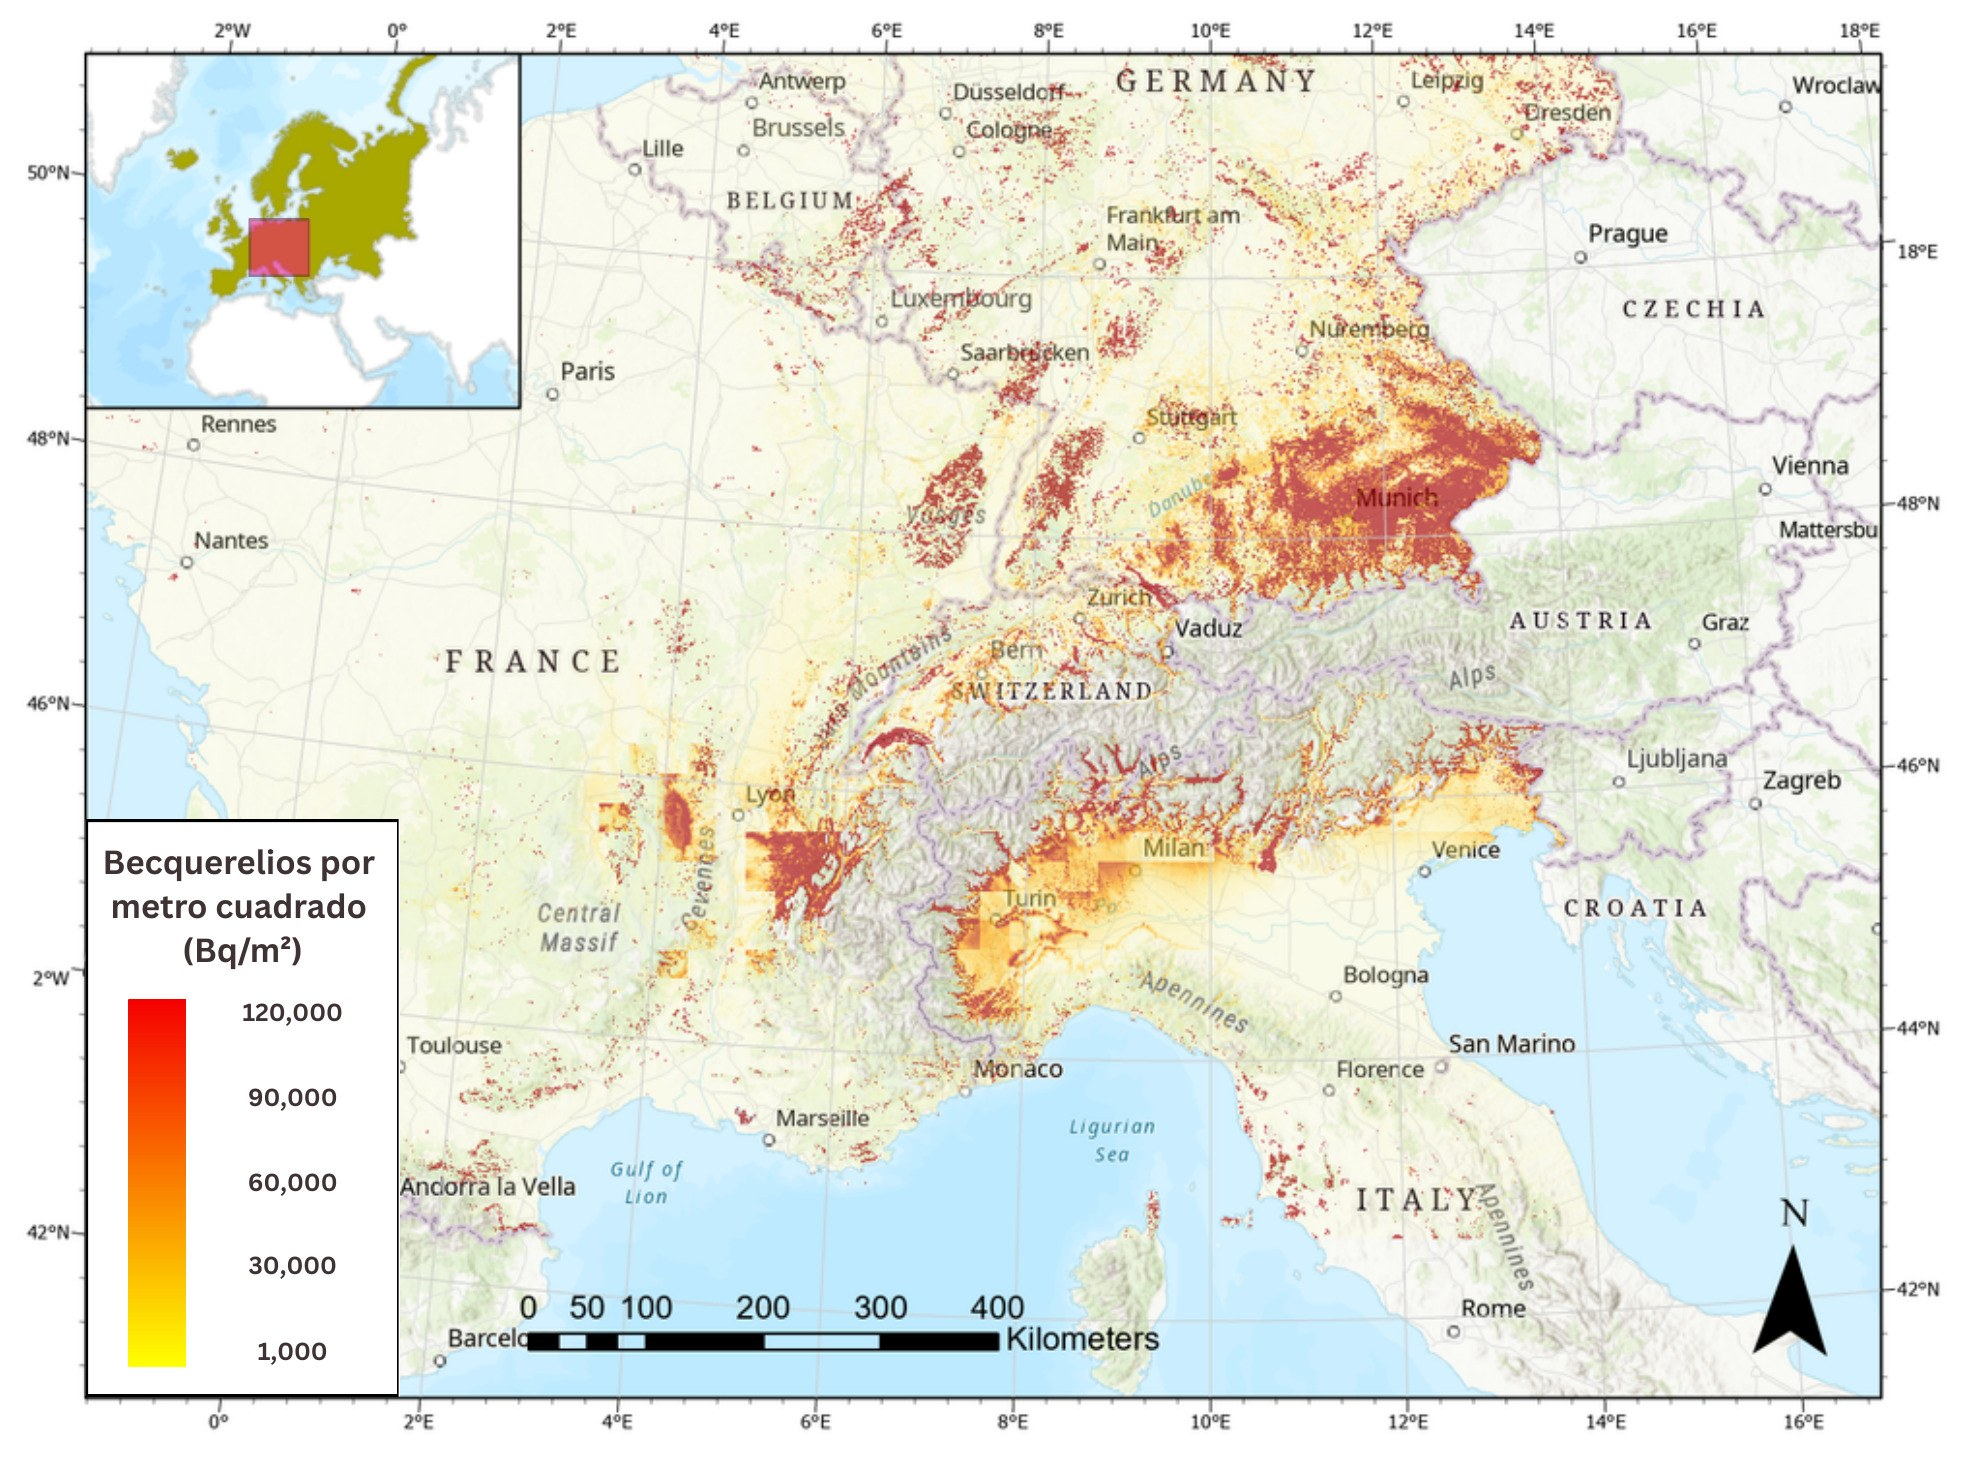
\includegraphics[width=0.78\textwidth]{f1_deposicion.jpg}
\caption{Deposici\'on inicial de $^{137}$Cs en Europa Central (mayo de 1986). La escala de color indica la actividad depositada, de 1,000 a 120,000~Bq/m$^2$.}
\label{fig:dep}
\end{figure*}

La ruptura del gradiente con la distancia se aprecia a escala urbana. M\'unich, a 1,379~km de Chernobyl, est\'a en el n\'ucleo de m\'axima deposici\'on, mientras que Viena, a solo 1,048~km, muestra valores bajos en la Fig.~\ref{fig:dep}, lo que concuerda con la escasa lluvia del este de Austria durante el paso de la nube~\cite{geosphere2026}.

\subsection{Barrera org\'afica}
Al superponer la deposici\'on sobre el relieve (Fig.~\ref{fig:oro}) se observa un estancamiento marcado de part\'iculas en las laderas septentrionales de los Alpes. Hacia la pen\'insula itálica y el Mediterr\'aneo los niveles bajan a valores m\'inimos. A\'un as\'i hay acumulaciones locales en algunos valles alpinos y en el piedemonte meridional, de modo que la cordillera parece modular la deposici\'on sin eliminarla. Esta lectura es visual: no se cuenta con datos de precipitaci\'on de 1986 para cuantificarla.

\begin{figure*}[t]
\centering
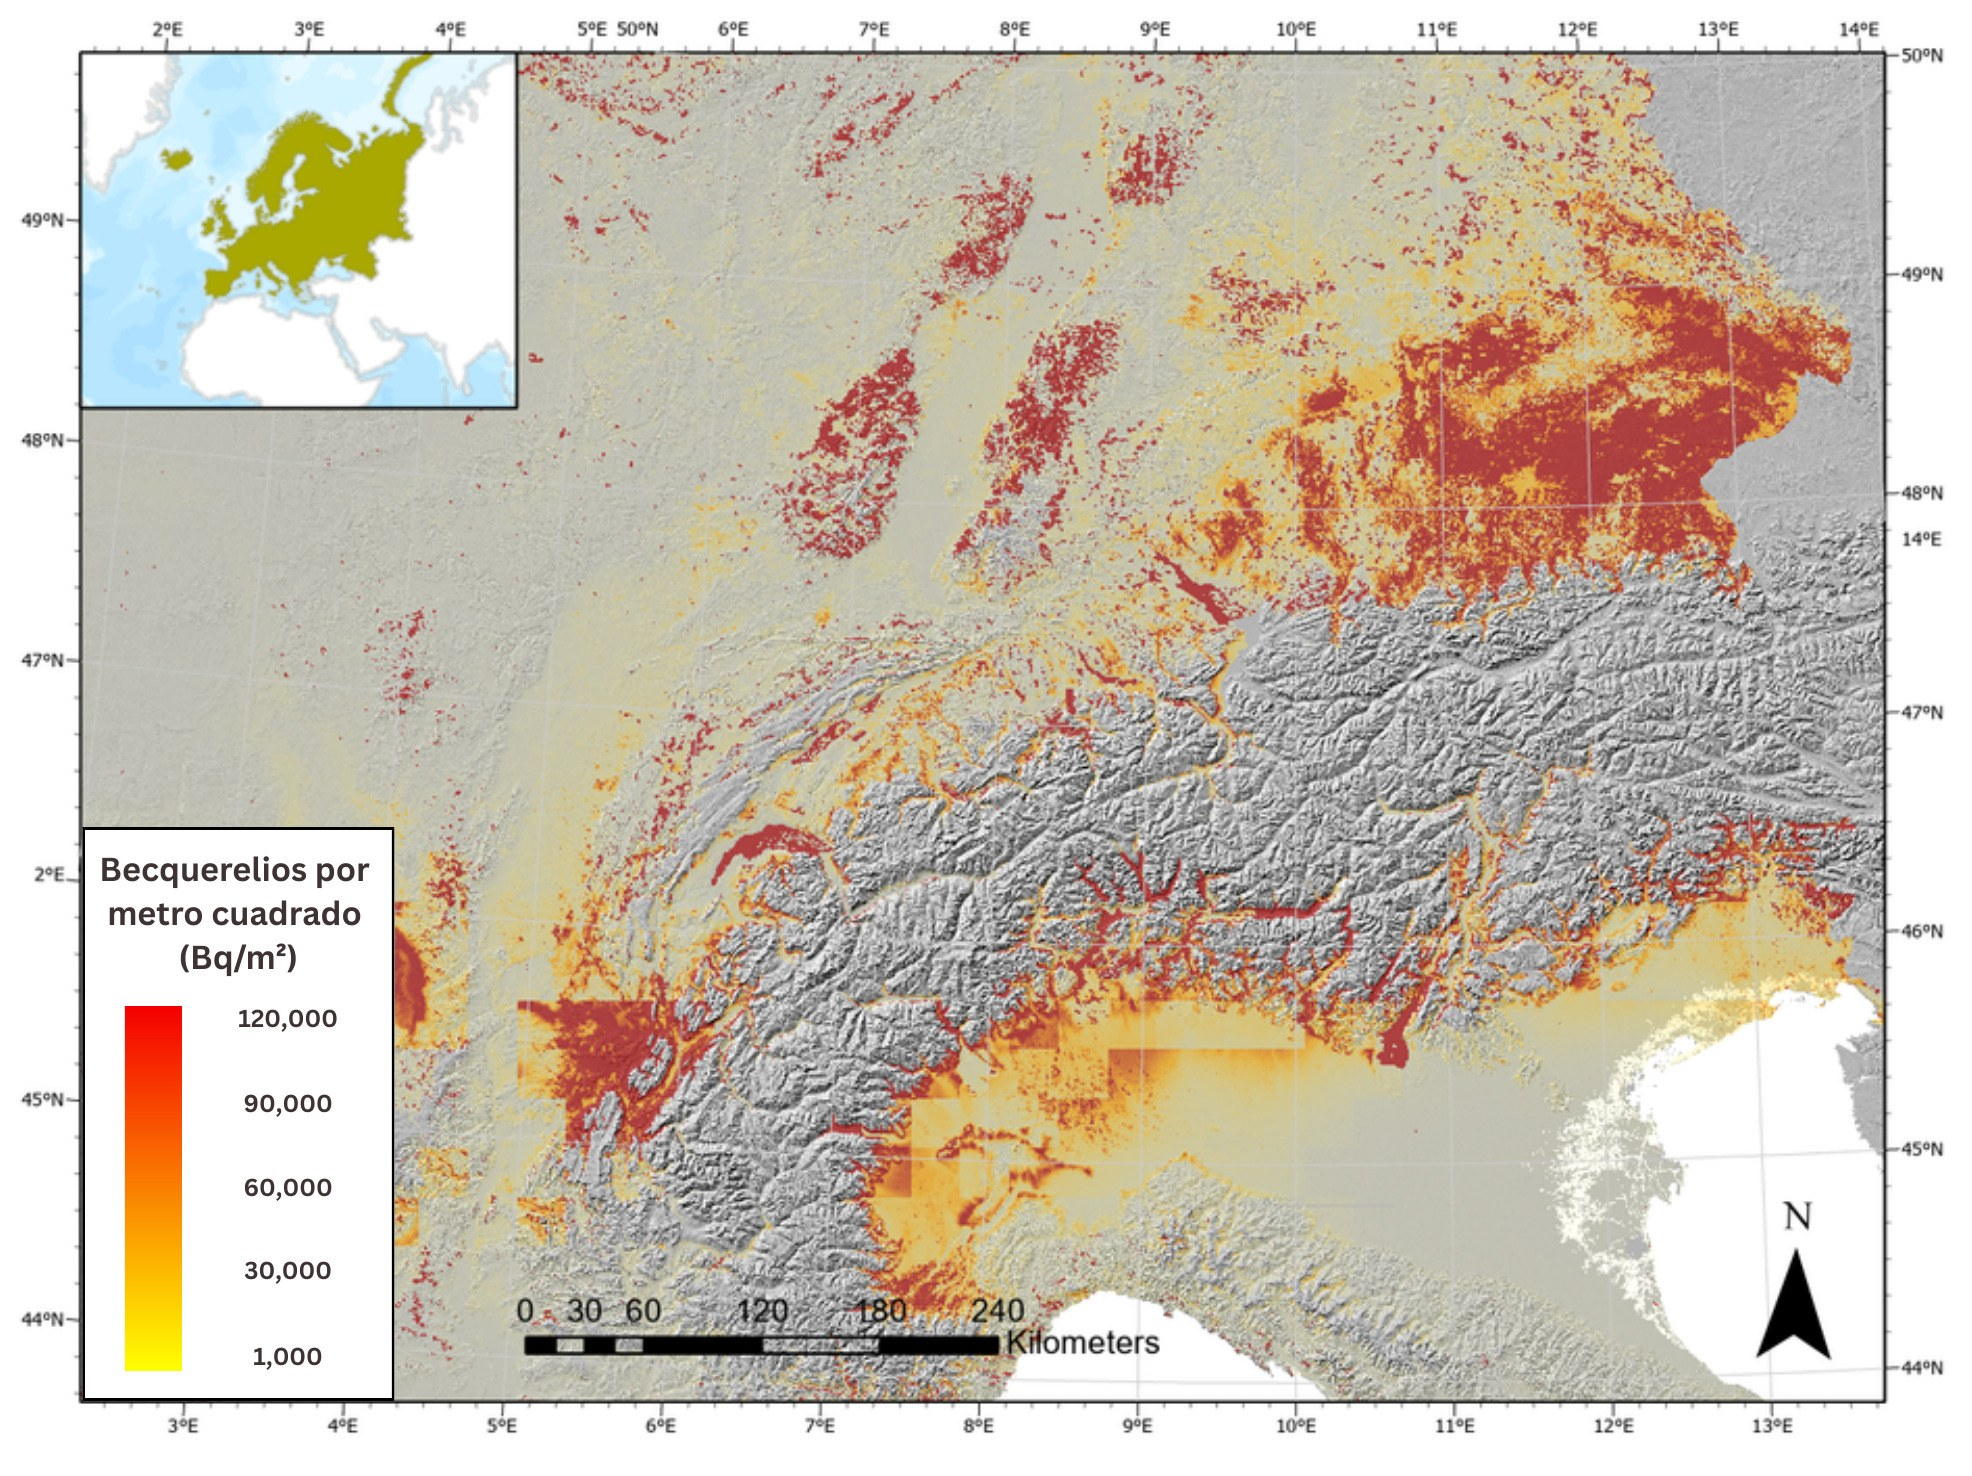
\includegraphics[width=0.78\textwidth]{f2_orografia.jpg}
\caption{Forzamiento orogr\'afico y posible efecto de barrera de los Alpes. Deposici\'on de $^{137}$Cs con 40~\% de transparencia sobre el relieve sombreado del DEM SRTM GL3.}
\label{fig:oro}
\end{figure*}

\subsection{Intensidad por pa\'is y distancia}
La Fig.~\ref{fig:paises} y la Tabla~\ref{tab:paises} resumen la intensidad media por pa\'is, ordenada por la distancia del centroide a Chernobyl. La clasificaci\'on sigue en parte la distancia: los tres pa\'ises m\'as cercanos (Rep\'ublica Checa, Austria y Eslovenia) est\'an en la clase m\'as alta. Hay, sin embargo, diferencias llamativas. Italia y Suiza tienen centroides a distancias casi iguales (1,660 y 1,671~km), pero Suiza, en su mayor parte al norte de la divisoria alpina, queda en la clase intermedia e Italia, a sotavento, en la m\'as baja. En Alemania, adem\'as, la media nacional atena los valores altos del sur, lo que muestra su heterogeneidad interna.

\begin{table}[t]
\centering
\caption{Intensidad media de $^{137}$Cs por pa\'is y distancia geod\'esica de su centroide a Chernobyl}
\label{tab:paises}
\begin{tabular}{lrc}
\toprule
Pa\'is & Distancia (km) & Clase (Bq/m$^2$)\\
\midrule
Rep\'ublica Checa & 1,061 & 28,000--120,000\\
Austria & 1,230 & 28,000--120,000\\
Eslovenia & 1,265 & 28,000--120,000\\
Alemania & 1,375 & 6,000--28,000\\
Italia & 1,660 & $<$\,6,000\\
Suiza & 1,671 & 6,000--28,000\\
Luxemburgo & 1,704 & $<$\,6,000\\
B\'elgica & 1,779 & $<$\,6,000\\
Francia\textsuperscript{a} & 2,079 & $<$\,6,000\\
\bottomrule
\multicolumn{3}{l}{\footnotesize \textsuperscript{a}Territorio metropolitano.}
\end{tabular}
\end{table}

\begin{figure}[t]
\centering
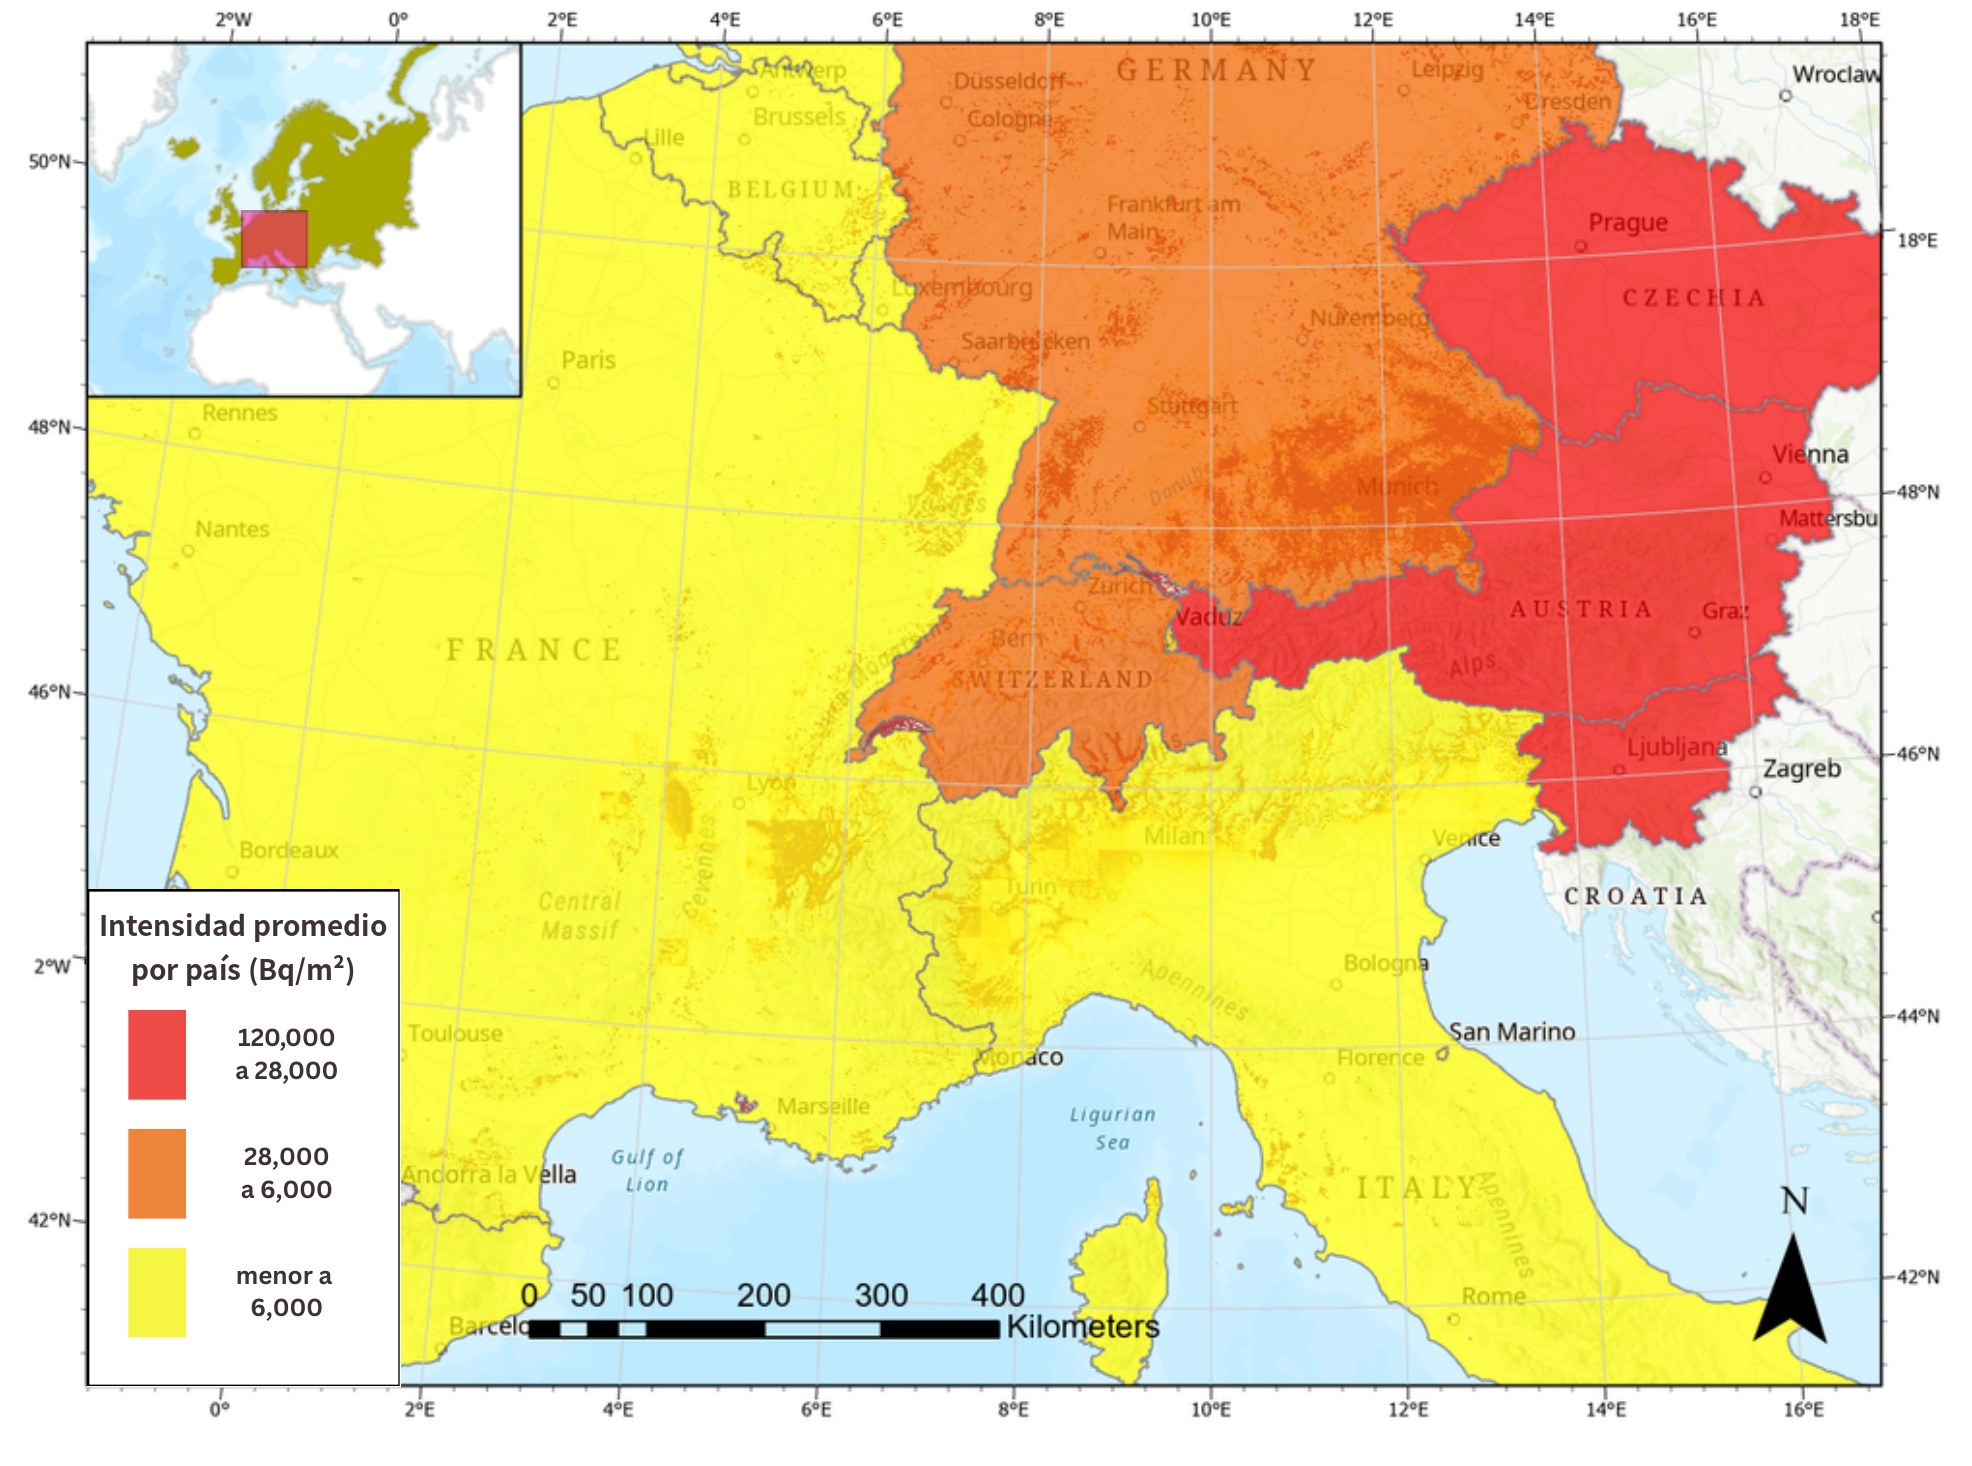
\includegraphics[width=\columnwidth]{f3_paises.jpg}
\caption{Intensidad media de $^{137}$Cs por pa\'is, obtenida con estad\'istica zonal.}
\label{fig:paises}
\end{figure}

\subsection{Evoluci\'on temporal}
Con (\ref{eq:decay}) el factor de decaimiento es 0.456 para mayo de 2020 y 0.397 para mayo de 2026: en 2020 quedaba el 45.6~\% del inventario inicial y en 2026 cerca del 40~\%, en l\'inea con la estimaci\'on de la BfS de que cerca del 60~\% del $^{137}$Cs ya decay\'o~\cite{bfs2026}. La Tabla~\ref{tab:decay} y la Fig.~\ref{fig:decay} muestran los valores de referencia. Los picos de 120,000~Bq/m$^2$ bajan a unos 54,800~Bq/m$^2$ en 2020 y seguir\'an por encima de 37~kBq/m$^2$ hasta cerca de 2037, 51~a\~nos despu\'es del accidente. En cambio, las zonas del l\'imite de 28,000~Bq/m$^2$ ya estaban por debajo de 13,000~Bq/m$^2$ en 2020.

\begin{table}[t]
\centering
\caption{Actividad remanente de $^{137}$Cs (Bq/m$^2$) por decaimiento f\'isico}
\label{tab:decay}
\begin{tabular}{lrrr}
\toprule
Referencia & 1986 & 2020 & 2026\\
\midrule
Pico m\'aximo & 120,000 & 54,775 & 47,695\\
L\'imite de clase superior & 28,000 & 12,781 & 11,129\\
L\'imite de clase inferior & 6,000 & 2,739 & 2,385\\
M\'inimo cartografiado & 1,000 & 456 & 397\\
\bottomrule
\end{tabular}
\end{table}

\begin{figure}[t]
\centering
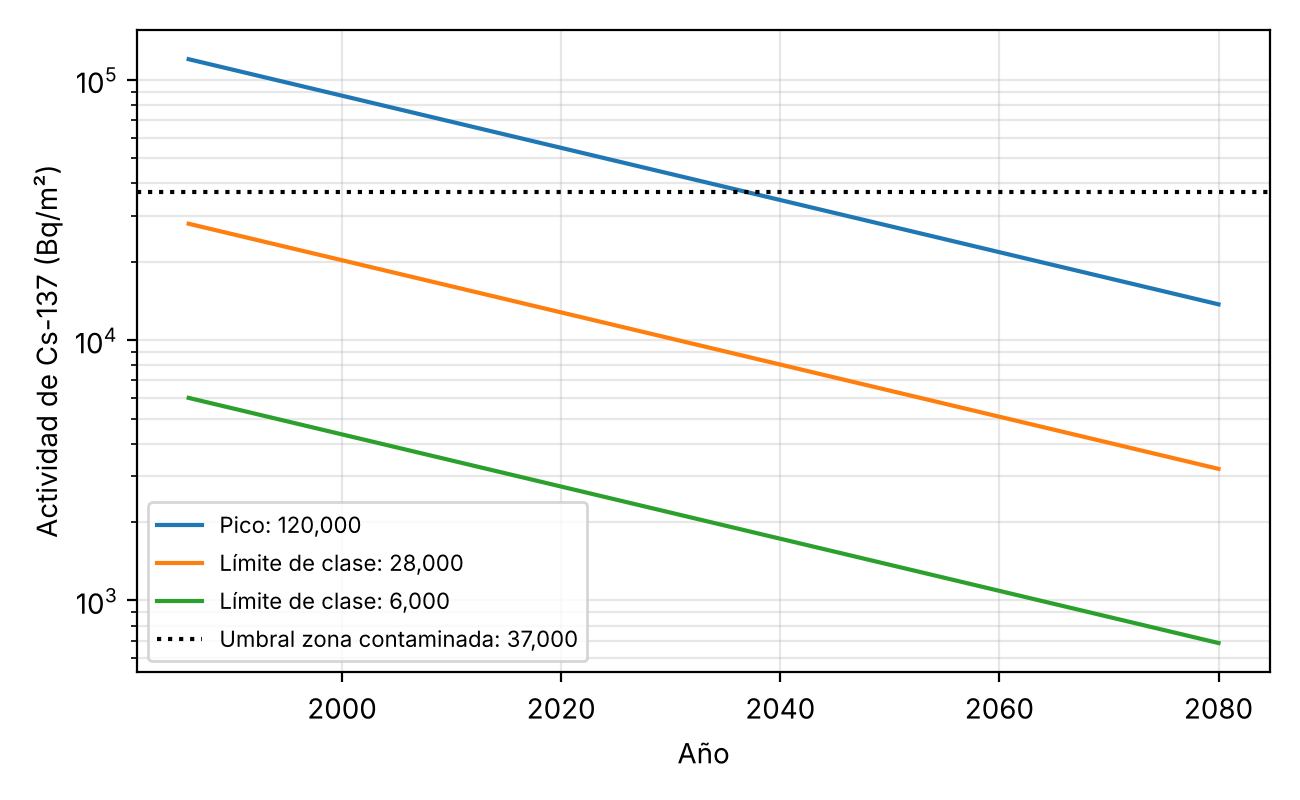
\includegraphics[width=\columnwidth]{f4_decaimiento.png}
\caption{Decaimiento f\'isico del $^{137}$Cs para el pico m\'aximo y los l\'imites de clase (escala logar\'itmica). La l\'inea punteada marca el umbral de 37~kBq/m$^2$ de las zonas contaminadas~\cite{iaea2006}.}
\label{fig:decay}
\end{figure}

\subsection{Revisi\'on con la literatura}
El orden relativo de los resultados es coherente con lo publicado. Seg\'un Izrael et al.~\cite{izrael1996}, Austria recibi\'o el 2.7~\% del $^{137}$Cs depositado en Europa y Alemania el 1.1~\%. Al dividir esas fracciones entre la superficie de cada pa\'is, la densidad media de Austria resulta unas 10.5 veces la de Alemania, lo que concuerda con su posici\'on en la Tabla~\ref{tab:paises}. Adem\'as, las medias provinciales de Alta Austria, Salzburgo y Carintia (59, 46 y 33~kBq/m$^2$)~\cite{oecd2002} caen en la clase m\'as alta.

En valores absolutos, en cambio, las medias nacionales parecen sobrestimadas. Bossew et al.~\cite{bossew2001}, con 2,115 puntos de muestreo, reportan para Austria una media de 21.0~kBq/m$^2$ (18.7~kBq/m$^2$ de Chernobyl), con m\'aximos cercanos a 200~kBq/m$^2$; esa media corresponder\'ia a la clase intermedia y no a la superior. Del mismo modo, combinada con el cociente de 10.5, la media de Alemania ser\'ia del orden de 2~kBq/m$^2$, por debajo del rango asignado; esta estimaci\'on indirecta es coherente con los valores menores de 4,000~Bq/m$^2$ que la BfS reporta para el norte del pa\'is~\cite{bfs2026}. Una causa probable es que las celdas por debajo de 1,000~Bq/m$^2$, el l\'imite inferior de la simbolog\'ia, se hayan tratado como celdas sin dato, de modo que el promedio solo incluy\'o \'areas contaminadas. Adem\'as, el tope de 120,000~Bq/m$^2$ viene de la simbolog\'ia y no de los datos, pues la literatura reporta m\'aximos locales mayores. Por ello las clases de la Tabla~\ref{tab:paises} deben leerse como un orden relativo entre pa\'ises m\'as que como valores absolutos.

\section{Caso de estudio: Laguna Verde, M\'exico}
\subsection{Contexto}
La Central Nucleoel\'ectrica de Laguna Verde, operada por la Comisi\'on Federal de Electricidad, est\'a en la costa del Golfo de M\'exico, en Veracruz. Tiene dos reactores de agua en ebullici\'on (BWR-5) de 777 y 775~MWe netos, que generan cerca del 4~\% de la electricidad del pa\'is~\cite{wna2026}. El PERE define una ZVP de 16~km de radio, donde la exposici\'on principal viene de la nube, y una ZVI de 80~km, donde predominan el consumo de agua y alimentos contaminados y el material depositado en los suelos~\cite{pere2011}.

La regi\'on est\'a dominada por dos reg\'imenes de viento: los alisios, que en verano traen aire h\'umedo del Golfo, y los nortes invernales, asociados a masas de aire polar que tambi\'en recogen humedad del Golfo~\cite{garcia2003,perez2018}. En la vertiente del Golfo la precipitaci\'on aumenta donde las monta\~nas son perpendiculares a los vientos dominantes, alcanza su m\'aximo entre 100 y 600~m de altitud y supera los 2,000~mm anuales en \'areas extensas~\cite{garcia2003}. La Sierra Madre Oriental desciende desde los 4,282~m del Cofre de Perote hasta el nivel del mar en unos 100~km, y la lluvia anual pasa de unos 1,600~mm en la planicie costera del sur a unos 620~mm en el Altiplano~\cite{perez2018}.

\subsection{Resultados morfoestructurales}
La Fig.~\ref{fig:lv} y la Tabla~\ref{tab:lv} muestran que Xalapa (56~km) y el puerto de Veracruz (67~km) est\'an dentro de la ZVI, y que el Cofre de Perote queda justo en su l\'imite (82~km). El perfil de la Fig.~\ref{fig:perf}(b), trazado hacia el Cofre de Perote y aproximadamente en la direcci\'on de los alisios, indica que el terreno sube de unos 170~m en la costa a cerca de 2,340~m a los 80~km, con una pendiente media de unos 27~m/km. En la misma malla, la vertiente norte de los Alpes (Fig.~\ref{fig:perf}(a)) sube unos 1,640~m entre $48^\circ$\,N y la cresta suavizada, en 110~km, es decir, unos 15~m/km. As\'i, la ZVI de Laguna Verde incluye una rampa orogr\'afica casi dos veces m\'as pronunciada que la que acompa\~n\'o la deposici\'on en el sur de Baviera.

\begin{figure}[t]
\centering
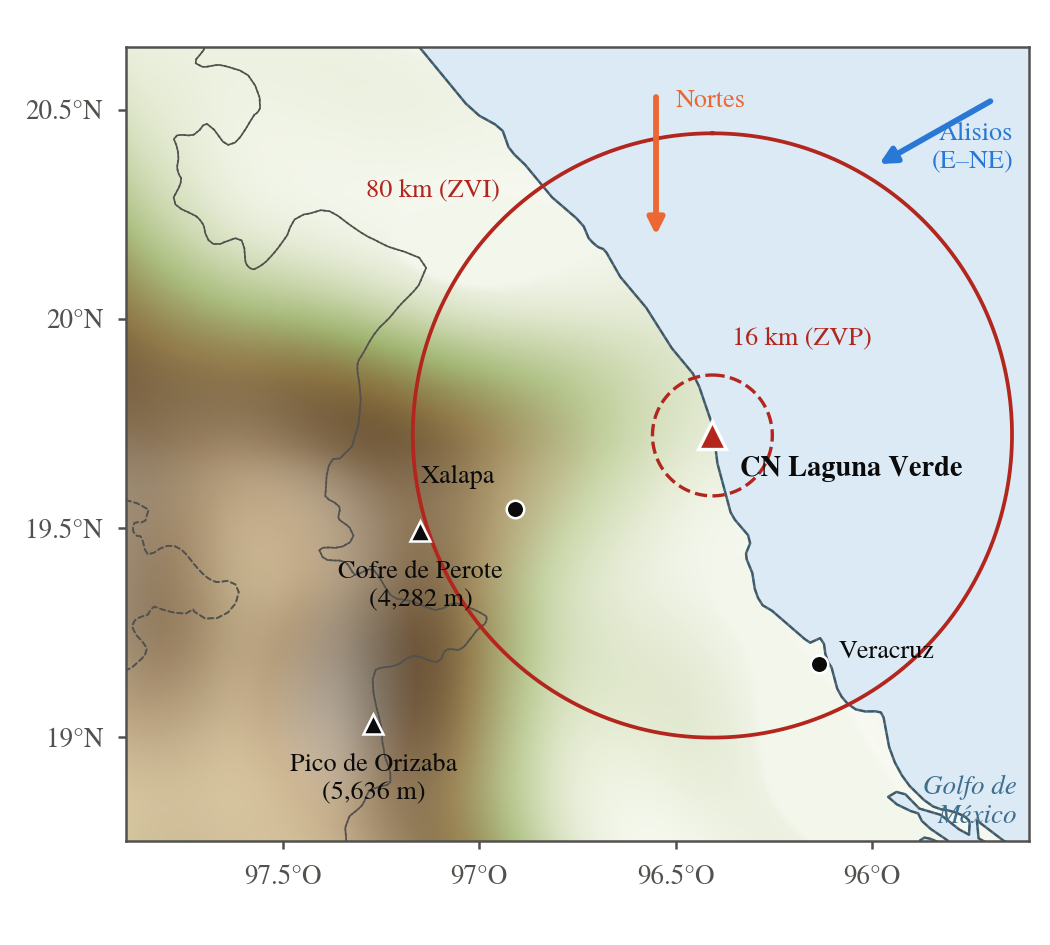
\includegraphics[width=\columnwidth]{f5_laguna_verde.png}
\caption{Entorno de la Central Nucleoel\'ectrica de Laguna Verde (CNLV) sobre la topograf\'ia ETOPO1 a $10'$~\cite{etopo1,fatiando}, con las zonas del PERE~\cite{pere2011} y los reg\'imenes de viento dominantes (representaci\'on cualitativa)~\cite{garcia2003}.}
\label{fig:lv}
\end{figure}

\begin{table}[t]
\centering
\caption{Localidades y relieves de referencia respecto a Laguna Verde}
\label{tab:lv}
\begin{tabular}{lrcc}
\toprule
Sitio & Dist. (km) & Acimut & Zona PERE\\
\midrule
Xalapa & 56 & 250$^\circ$ & ZVI\\
Veracruz (puerto) & 67 & 155$^\circ$ & ZVI\\
Cofre de Perote & 82 & 252$^\circ$ & L\'imite ZVI\\
Pico de Orizaba & 119 & 230$^\circ$ & Fuera\\
\bottomrule
\end{tabular}
\end{table}

\begin{figure}[t]
\centering
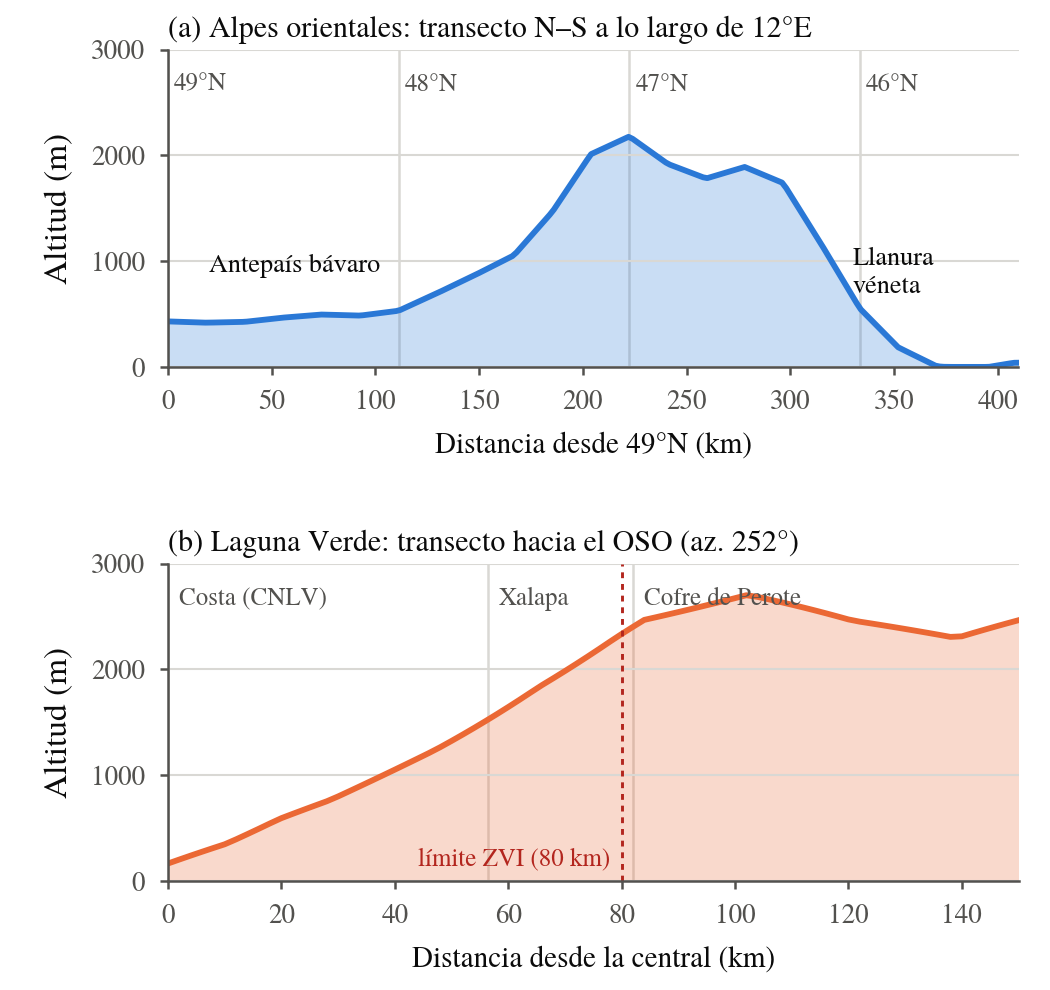
\includegraphics[width=\columnwidth]{f6_perfiles.png}
\caption{Perfiles topogr\'aficos de la misma malla ETOPO1 a $10'$~\cite{etopo1,fatiando}: (a) Alpes orientales a lo largo de $12^\circ$\,E; (b) desde Laguna Verde hacia el Cofre de Perote. La resoluci\'on suaviza las cumbres; el Cofre de Perote alcanza 4,282~m~\cite{perez2018}.}
\label{fig:perf}
\end{figure}

\subsection{Escenarios de dispersi\'on}
Por analog\'ia con el caso alpino se plantean dos escenarios cualitativos. Con alisios del este-noreste, una pluma ser\'ia llevada hacia el oeste-suroeste, justo sobre la rampa que conduce a Xalapa y al Cofre de Perote; en ese trayecto el ascenso forzado intensifica la precipitaci\'on~\cite{garcia2003}, por lo que podr\'ian formarse n\'ucleos de deposici\'on h\'umeda dentro de la ZVI, an\'alogos a los del piedemonte norte de los Alpes. Con nortes, en cambio, el transporte ser\'ia hacia el sur, paralelo a la costa y hacia el puerto de Veracruz, con la precipitaci\'on propia de esos eventos. Ambos escenarios son hip\'otesis que requieren validaci\'on con modelos de dispersi\'on atmosf\'erica.

\section{Discusi\'on}
Los resultados indican que la vulnerabilidad territorial ante una emergencia nuclear no depende solo de la cercan\'ia a la fuente. En Europa Central, la combinaci\'on de lluvia durante el paso de la nube y un relieve perpendicular al flujo parece haber concentrado la deposici\'on a m\'as de 1,000~km de Chernobyl, mientras que zonas m\'as cercanas pero secas, como el este de Austria, recibieron menos. Por eso los modelos de riesgo basados solo en c\'irculos de distancia podr\'ian subestimar la exposici\'on a barlovento y sobrestimarla a sotavento. En Laguna Verde, la ZVI incluye una rampa orogr\'afica pronunciada y expuesta a vientos h\'umedos del Golfo en verano e invierno; la planificaci\'on de emergencias podr\'ia complementarse con mapas que integren relieve, climatolog\'ia de vientos y precipitaci\'on adem\'as de la distancia.

El trabajo tiene varias limitaciones:
\begin{itemize}
\item el efecto orogr\'afico en Europa se evalu\'o por correlaci\'on visual, sin datos de precipitaci\'on de 1986;
\item los promedios por pa\'is podr\'ian estar sesgados al alza, como se discuti\'o en la revisi\'on con la literatura;
\item la evoluci\'on temporal considera solo el decaimiento f\'isico;
\item el an\'alisis de Laguna Verde usa topograf\'ia a $10'$, que suaviza el relieve, y escenarios de viento cualitativos.
\end{itemize}
Como trabajo futuro se propone recalcular la estad\'istica zonal incluyendo todas las celdas; cuantificar la relaci\'on entre deposici\'on y precipitaci\'on con bases de mediciones de 1986~\cite{evangeliou2016}; repetir el an\'alisis de Laguna Verde con el DEM SRTM GL3 y la climatolog\'ia local de vientos; y simular escenarios de liberaci\'on con modelos lagrangianos como HYSPLIT~\cite{stein2015} o FLEXPART~\cite{pisso2019}.

\section{Conclusiones}
Con la metodolog\'ia descrita, la deposici\'on de $^{137}$Cs tras Chernobyl muestra una ruptura del gradiente con la distancia, con valores de hasta 120,000~Bq/m$^2$ a m\'as de 1,000~km de la fuente. La distribuci\'on es coherente con un efecto de barrera de los Alpes, que concentr\'o material en su vertiente norte y lo redujo hacia el sur; as\'i, Italia y Suiza, a distancias casi iguales, quedan en clases distintas, aunque esta lectura es visual y requiere datos de precipitaci\'on para confirmarse. El decaimiento f\'isico deja el 45.6~\% del inventario en 2020 y los picos seguir\'ian sobre el umbral de zona contaminada hasta cerca de 2037. Al trasladar el an\'alisis a M\'exico, la zona de ingesti\'on de Laguna Verde abarca una rampa orogr\'afica expuesta a los alisios, por lo que incorporar el relieve a la evaluaci\'on del riesgo radiol\'ogico ayudar\'ia a delimitar las zonas vulnerables.

\section*{Disponibilidad de c\'odigo}
El c\'odigo que reproduce las distancias de la Tabla~\ref{tab:paises}, los valores de las Tablas~\ref{tab:decay} y~\ref{tab:lv} y la Fig.~\ref{fig:decay} est\'a en \url{https://github.com/ianachlisv-rgb/cesio137-chernobyl-sig}. El atlas de De Cort et al.~\cite{decort1998} no est\'a disponible en formato digital; las clases de la Tabla~\ref{tab:paises} y los perfiles de la Fig.~\ref{fig:perf} provienen del procesamiento del autor sobre la matriz de deposici\'on y la malla ETOPO1 descritas arriba.

\begin{thebibliography}{99}
\bibitem{oecd2002} OECD Nuclear Energy Agency, ``The release, dispersion, deposition and behaviour of radionuclides,'' en \textit{Chernobyl: Assessment of Radiological and Health Impacts. 2002 Update of Chernobyl: Ten Years On}, cap.~II. Par\'is: OECD/NEA, 2002.
\bibitem{pearce2008} A. Pearce, ``Recommended nuclear decay data,'' National Physical Laboratory, Teddington, Reino Unido, NPL Rep. IR 6, ene. 2008.
\bibitem{iaea2006} International Atomic Energy Agency, \textit{Environmental Consequences of the Chernobyl Accident and their Remediation: Twenty Years of Experience}, Radiological Assessment Reports Series. Viena: IAEA, 2006.
\bibitem{izrael1996} Yu.~A. Izrael \textit{et al.}, ``The atlas of caesium-137 contamination of Europe after the Chernobyl accident,'' en \textit{Proc. 1st Int. Conf. The Radiological Consequences of the Chernobyl Accident}, Minsk, Bielorrusia, mar. 1996, pp.~1--10.
\bibitem{garcia2003} E. Garc\'ia, ``Distribuci\'on de la precipitaci\'on en la Rep\'ublica Mexicana,'' \textit{Investigaciones Geogr\'aficas}, no.~50, pp.~67--76, 2003.
\bibitem{kalkan2021} S.~K. Kalkan \textit{et al.}, ``Deposition of $^{137}$Cs and precipitation distribution in Vojvodina, Northern Serbia after the Chernobyl accident,'' \textit{Chemosphere}, vol.~264, art. 128471, 2021, doi: 10.1016/j.chemosphere.2020.128471.
\bibitem{geosphere2026} GeoSphere Austria, ``40 years since the Chernobyl nuclear disaster,'' 2026. [En l\'inea]. Disponible: \url{https://www.geosphere.at}
\bibitem{decort1998} M. De Cort \textit{et al.}, \textit{Atlas of Caesium Deposition on Europe after the Chernobyl Accident}, EUR 16733 EN. Luxemburgo: European Commission, Joint Research Centre, 1998.
\bibitem{srtm2013} NASA JPL, ``NASA Shuttle Radar Topography Mission Global 3 arc second (SRTMGL3 v003),'' NASA EOSDIS Land Processes DAAC, 2013. [Conjunto de datos]. Accedido v\'ia OpenTopography. doi: 10.5067/MEaSUREs/SRTM/SRTMGL3.003.
\bibitem{ne10} Natural Earth, ``Natural Earth vector data, 1:10m cultural and physical themes.'' [Conjunto de datos]. Disponible: \url{https://www.naturalearthdata.com}
\bibitem{etopo1} C. Amante y B.~W. Eakins, ``ETOPO1 1 arc-minute global relief model: Procedures, data sources and analysis,'' NOAA Tech. Memo. NESDIS NGDC-24, 2009, doi: 10.7289/V5C8276M.
\bibitem{fatiando} Fatiando a Terra Project, ``Earth topography grid at 10 arc-minute resolution,'' v1, Zenodo, 2022. [Conjunto de datos]. doi: 10.5281/zenodo.5882203.
\bibitem{pere2011} Sistema Nacional de Protecci\'on Civil, ``Plan de Emergencia Radiol\'ogica Externo de la Central Nucleoel\'ectrica Laguna Verde (PERE),'' M\'exico, 2011.
\bibitem{bfs2026} Bundesamt f\"ur Strahlenschutz (BfS), ``Environmental contamination and other consequences of the Chornobyl reactor accident,'' 2026. [En l\'inea]. Disponible: \url{https://www.bfs.de}
\bibitem{bossew2001} P. Bossew, M. Ditto, T. Falkner, E. Henrich, K. Kienzl y U. Rappelsberger, ``Contamination of Austrian soil with caesium-137,'' \textit{J. Environ. Radioact.}, vol.~55, no.~2, pp.~187--194, 2001.
\bibitem{wna2026} World Nuclear Association, ``Nuclear power in Mexico,'' 2026. [En l\'inea]. Disponible: \url{https://world-nuclear.org}
\bibitem{perez2018} M. P\'erez M\'endez, ``La lluvia en el centro de Veracruz,'' \textit{Ciencia UV}, Universidad Veracruzana, 2018.
\bibitem{evangeliou2016} N. Evangeliou \textit{et al.}, ``Reconstructing the Chernobyl Nuclear Power Plant (CNPP) accident 30 years after. A unique database of air concentration and deposition measurements over Europe,'' \textit{Environ. Pollut.}, vol.~216, pp.~408--418, 2016, doi: 10.1016/j.envpol.2016.05.030.
\bibitem{stein2015} A.~F. Stein, R.~R. Draxler, G.~D. Rolph, B.~J.~B. Stunder, M.~D. Cohen y F. Ngan, ``NOAA's HYSPLIT atmospheric transport and dispersion modeling system,'' \textit{Bull. Amer. Meteor. Soc.}, vol.~96, no.~12, pp.~2059--2077, 2015, doi: 10.1175/BAMS-D-14-00110.1.
\bibitem{pisso2019} I. Pisso \textit{et al.}, ``The Lagrangian particle dispersion model FLEXPART version 10.4,'' \textit{Geosci. Model Dev.}, vol.~12, pp.~4955--4997, 2019, doi: 10.5194/gmd-12-4955-2019.
\end{thebibliography}

\end{document}
